%%
%% SC26 Submission - Cascade: Content-Addressed Tiered KV Cache Storage for HPC-Scale LLM Inference
%%
\documentclass[conference]{IEEEtran}
\IEEEoverridecommandlockouts

%% Packages
\usepackage{amsmath}
\usepackage{cite}
\usepackage{graphicx}
\usepackage{amsfonts}
\usepackage{multirow}
\usepackage{xspace}
\usepackage{pifont}
\usepackage[caption=false]{subfig}
\usepackage{float}
\usepackage{url}
\usepackage{array}
\usepackage{booktabs}
\usepackage{enumitem}
\usepackage{tikz}
\usetikzlibrary{fit,shapes,arrows,positioning}
\usepackage{xcolor}
\usepackage{colortbl}
\usepackage{caption}
\usepackage{algorithm}
\usepackage{algorithmic}

%% Space-saving adjustments
\setlength{\tabcolsep}{2pt}
\setlength{\textfloatsep}{4pt plus 1.0pt minus 2.0pt}
\setlength{\floatsep}{4pt plus 1.0pt minus 2.0pt}
\setlength{\intextsep}{4pt plus 1.0pt minus 2.0pt}
\setlength{\dbltextfloatsep}{4pt plus 1.0pt minus 2.0pt}
\setlength{\dblfloatsep}{4pt plus 1.0pt minus 2.0pt}
\setlength{\abovedisplayskip}{3pt}
\setlength{\belowdisplayskip}{3pt}
\setlength{\abovecaptionskip}{2pt}
\setlength{\belowcaptionskip}{0pt}
\renewcommand{\arraystretch}{0.85}

%% Commands
\newcommand{\Cascade}{\textsc{Cascade}\xspace}
\newcommand{\cmark}{{\color{green!70!black}\ding{51}}}
\newcommand{\xmark}{{\color{red!80!black}\ding{55}}}
\newcommand{\pmark}{{\color{orange!80!black}$\triangle$}}

\begin{document}

\title{\Cascade: Content-Addressed Tiered KV Cache Storage\\for HPC-Scale LLM Inference}

%% Anonymous author block for double-blind review
\author{}

\maketitle

\begin{abstract}
Large language model (LLM) inference at HPC scale requires efficient KV cache management to support long contexts and multi-node serving.
Existing KV cache storage systems such as LMCache and Mooncake are optimized for datacenter environments with local NVMe storage and session-specific block addressing, limiting cross-session deduplication and HPC deployment.
This paper presents \Cascade, a four-tier content-addressed KV cache storage system designed for HPC environments.
\Cascade introduces: (1) \textbf{content-addressed block identification} via SHA-256 hashing for automatic deduplication of shared prefixes across sessions,
(2) a \textbf{four-tier storage hierarchy} (GPU HBM $\rightarrow$ Local DRAM $\rightarrow$ Remote DRAM via MPI $\rightarrow$ Lustre PFS) with semantic-aware eviction that protects frequently-shared prefix blocks,
and (3) \textbf{HPC-optimized data placement} using aggregated files with Lustre striping to overcome metadata overhead.
Our key insight is that content-addressed deduplication combined with an MPI-based global address space achieves significant storage savings for multi-tenant LLM workloads sharing system prompts.

\textbf{[TODO: Finalize evaluation numbers after experiments on Perlmutter]}

Evaluated on NERSC Perlmutter with up to 256 nodes, \Cascade targets XX\% higher cache hit rates and XX$\times$ lower time-to-first-token compared to LMCache and other datacenter-optimized baselines.
\end{abstract}

\begin{IEEEkeywords}
High Performance Computing, Large Language Models, KV Cache, Content-Addressed Storage, Distributed Inference, Deduplication
\end{IEEEkeywords}

\section{Introduction}
\label{sec:introduction}

Large language models (LLMs) have become the foundation of modern AI applications,
from conversational agents to code generation and scientific discovery~\cite{openai2023gpt4, touvron2023llama}.
As LLM inference scales to serve millions of users across increasingly long contexts,
the key-value (KV) cache has emerged as a critical bottleneck.
The KV cache stores attention states from previously processed tokens,
enabling efficient autoregressive generation without recomputation.
For models like LLaMA-70B with Grouped Query Attention (GQA) and 128K context windows,
the KV cache alone can consume tens of gigabytes per request,
creating significant memory pressure.

The challenge of KV cache management has driven significant research in datacenter environments.
Systems like vLLM~\cite{kwon2023vllm} introduced PagedAttention for memory-efficient KV cache allocation,
while LMCache~\cite{lmcache2024} and Mooncake~\cite{qin2024mooncake} enable multi-tier caching with local NVMe as the primary offloading tier.
However, these systems share a critical limitation: \textbf{session-specific block addressing}.
When multiple sessions share identical system prompts (e.g., ``You are a helpful AI assistant...''),
existing systems store and retrieve separate KV cache copies for each session,
missing obvious deduplication opportunities.

Furthermore, HPC systems present a \emph{fundamentally different storage architecture} than datacenters:

\begin{itemize}[leftmargin=*,nosep]
    \item \textbf{No local NVMe}: NERSC Perlmutter compute nodes lack local SSDs;
    the only persistent storage is the Lustre parallel file system.
    \item \textbf{Shared parallel file system}: Lustre provides high aggregate bandwidth (7.8 TB/s read)
    but incurs severe metadata overhead for small-file operations.
    \item \textbf{High-bandwidth interconnect}: Slingshot-11 provides 100 GB/s per node (4 $\times$ 25 GB/s NICs),
    enabling efficient cross-node KV cache sharing via MPI.
\end{itemize}

When existing KV cache systems are naively deployed on HPC systems,
they suffer significant performance degradation.
Our measurements show that LMCache-style per-file storage incurs
up to \textbf{29$\times$ lower read throughput} on Lustre compared to aggregated approaches
due to metadata operations.

\noindent\textbf{Key Insight: Content-Addressed Deduplication.}
We observe that in production LLM serving scenarios, 20-100 system prompts are shared across thousands of sessions.
If KV cache blocks are identified by their \emph{content hash} rather than session ID,
blocks containing identical prefixes are automatically deduplicated.
This insight, combined with HPC-native storage optimizations, motivates \Cascade.

\noindent\textbf{Contributions.} This paper presents \Cascade, a content-addressed tiered KV cache storage system for HPC.
Our contributions include:

\begin{enumerate}[leftmargin=*,nosep]
    \item \textbf{Content-Addressed Block Identification}:
    We compute block IDs via SHA-256 hashing of KV tensor content,
    enabling automatic deduplication of shared prefixes across sessions
    without explicit coordination.

    \item \textbf{Four-Tier HPC Storage Hierarchy}:
    We design a four-tier hierarchy (GPU HBM $\rightarrow$ Local DRAM via \texttt{/dev/shm} $\rightarrow$ Remote DRAM via MPI $\rightarrow$ Lustre PFS)
    with semantic-aware eviction that protects frequently-referenced prefix blocks.

    \item \textbf{HPC-Optimized Data Placement}:
    We demonstrate that aggregated single-file storage with Lustre striping (16 OSTs, 4MB stripe size)
    achieves up to 29$\times$ better throughput than per-file approaches,
    and develop rank-specific file naming to eliminate lock contention.

    \item \textbf{MPI-Based Global Address Space}:
    We leverage Cray MPICH on Slingshot-11 for efficient KV block transfer between nodes,
    creating a distributed cache that scales with node count.

    \item \textbf{Comprehensive Evaluation}:
    We evaluate \Cascade on Perlmutter with configurations up to 256 nodes,
    comparing against LMCache and other baselines.
    \textbf{[TODO: Add specific performance numbers]}
\end{enumerate}

The remainder of this paper is organized as follows.
Section~\ref{sec:background} provides background on KV cache management and HPC storage.
Section~\ref{sec:design} presents the \Cascade design.
Section~\ref{sec:evaluation} evaluates \Cascade on Perlmutter.
Section~\ref{sec:related} discusses related work.
Section~\ref{sec:discussion} addresses limitations.
Section~\ref{sec:conclusion} concludes.

\section{Background and Motivation}
\label{sec:background}

\subsection{KV Cache in LLM Inference}

Transformer-based LLMs use the attention mechanism to capture token dependencies.
During autoregressive generation, each new token attends to all previous tokens,
requiring key and value tensors for the entire context.
To avoid quadratic recomputation, systems cache these key-value pairs (the ``KV cache'').

For a model with $L$ layers, $H_{kv}$ key-value heads (with GQA), and head dimension $D$,
the KV cache size per token is:
\begin{equation}
    \text{KV}_\text{size} = 2 \times L \times H_{kv} \times D \times \text{precision}
\end{equation}

For LLaMA-2-70B with GQA ($L=80$, $H_{kv}=8$, $D=128$) in FP16,
this amounts to:
\begin{equation}
    2 \times 80 \times 8 \times 128 \times 2 = 327,680 \text{ bytes} \approx 320\text{KB/token}
\end{equation}

With a 128K context window, the KV cache reaches approximately 40GB per request.
For multi-tenant serving with hundreds of concurrent requests, aggregate KV cache demand
far exceeds available GPU memory.

\subsection{Existing KV Cache Storage Systems}

\textbf{vLLM}~\cite{kwon2023vllm} introduced PagedAttention,
managing KV cache as fixed-size pages (typically 16-256 tokens) to reduce memory fragmentation.
However, vLLM stores KV cache entirely in GPU memory, limiting context lengths.

\textbf{LMCache}~\cite{lmcache2024} extends PagedAttention with a multi-tier storage hierarchy:
GPU HBM $\rightarrow$ CPU DRAM $\rightarrow$ local NVMe $\rightarrow$ remote storage.
Each KV block is stored as a separate file with a \emph{session-specific} block ID,
preventing cross-session deduplication.

\textbf{Mooncake}~\cite{qin2024mooncake} optimizes for disaggregated storage,
using RDMA to transfer KV blocks between prefill and decode clusters.
It assumes dedicated NVMe pools for KV cache persistence.

\textbf{Common limitations:}
\begin{enumerate}[leftmargin=*,nosep]
    \item \textbf{Session-specific addressing}: Block IDs include session/request identifiers,
    preventing deduplication of identical content across sessions.
    \item \textbf{NVMe dependency}: Local NVMe assumed as primary offloading tier (3-6 GB/s).
    \item \textbf{Per-file storage}: Fine-grained eviction via separate files per block,
    which incurs severe metadata overhead on parallel file systems.
\end{enumerate}

\subsection{HPC Storage Architecture: Perlmutter}

NERSC's Perlmutter represents a modern HPC storage architecture:

\textbf{Compute nodes:} 1,536 GPU nodes, each with 4 NVIDIA A100-40GB GPUs,
AMD EPYC 7763 (64 cores), and 256GB DRAM.
\textbf{Critically: no local NVMe storage.}

\textbf{Parallel file system:} The Lustre-based \texttt{\$SCRATCH} provides:
\begin{itemize}[leftmargin=*,nosep]
    \item 44 PB capacity, 7.8 TB/s aggregate read bandwidth
    \item All-flash architecture with 4M+ IOPS
    \item Multi-MDT (Metadata Target) for improved metadata scalability
    \item Stripe-based data distribution across OSTs
\end{itemize}

\textbf{Node-local storage:} \texttt{/dev/shm}, a tmpfs backed by DRAM ($\sim$128GB available).

\textbf{Interconnect:} Slingshot-11 provides 100 GB/s per node (4 NICs $\times$ 25 GB/s),
with Cray MPICH optimized for the fabric.

\subsection{The Mismatch Problem}

When datacenter KV cache systems are deployed on HPC systems,
several mismatches cause severe performance degradation:

\textbf{1. Per-file storage overhead on Lustre:}
LMCache stores each KV block as a separate file.
On Lustre, each file operation involves MDS (Metadata Server) RPCs, introducing 10-50ms latency.
Table~\ref{tab:lustre-overhead} shows our measurements on Perlmutter:
for 42KB blocks (32 tokens, LMCache default), per-file storage achieves only 233 MB/s read
versus 6.8 GB/s for aggregated access---a \textbf{29$\times$ slowdown}.

\begin{table}[t]
\centering
\footnotesize
\caption{Per-file vs. aggregated storage throughput on Perlmutter Lustre (100 blocks).
Per-file mimics LMCache; aggregated mimics \Cascade.}
\label{tab:lustre-overhead}
\begin{tabular}{lrrr}
\toprule
\textbf{Block Size} & \textbf{Per-file} & \textbf{Aggregated} & \textbf{Speedup} \\
\midrule
\multicolumn{4}{l}{\textit{Write Throughput}} \\
42 KB (LMCache) & 61 MB/s & 766 MB/s & 12.6$\times$ \\
256 KB (\Cascade) & 291 MB/s & 971 MB/s & 3.3$\times$ \\
1 MB & 598 MB/s & 1,016 MB/s & 1.7$\times$ \\
\midrule
\multicolumn{4}{l}{\textit{Read Throughput}} \\
42 KB (LMCache) & 233 MB/s & 6,836 MB/s & \textbf{29.3$\times$} \\
256 KB (\Cascade) & 1,298 MB/s & 7,582 MB/s & 5.8$\times$ \\
1 MB & 3,211 MB/s & 7,962 MB/s & 2.5$\times$ \\
\bottomrule
\end{tabular}
\end{table}

\textbf{2. Missing NVMe tier:}
Without local NVMe, systems must choose between:
(1) DRAM-only caching ($\sim$128GB limit per node),
(2) Direct Lustre access (high latency), or
(3) Remote memory via network.

\textbf{3. Missed deduplication opportunity:}
In production LLM serving, 20-100 system prompts are shared across thousands of sessions.
Session-specific block IDs prevent leveraging this redundancy.

\subsection{Opportunity: Content-Addressed HPC-Native KV Cache}

Our key observations that motivate \Cascade:

\begin{enumerate}[leftmargin=*,nosep]
    \item \textbf{Content-level deduplication}:
    If block IDs are derived from content hash (SHA-256),
    identical prefixes automatically map to the same block,
    reducing storage and improving cache hit rates.

    \item \textbf{High-bandwidth interconnect}:
    Slingshot-11 at 100 GB/s per node enables efficient remote DRAM access,
    creating a third tier between local DRAM and Lustre.

    \item \textbf{Aggregated file storage}:
    Combining multiple blocks into large files (4-16 MB) with Lustre striping
    amortizes metadata costs and achieves near-maximum bandwidth.

    \item \textbf{MPI for tensor transfer}:
    Cray MPICH on Slingshot is highly optimized;
    for point-to-point KV block transfers, MPI matches or exceeds NCCL.
\end{enumerate}

These observations motivate \Cascade's content-addressed, four-tier design.

\section{Design}
\label{sec:design}

\Cascade is a content-addressed tiered KV cache storage system designed for HPC environments.
Figure~\ref{fig:architecture} shows the overall architecture.
We describe each component in detail.

\begin{figure*}[t]
    \centering
    \includegraphics[width=0.95\textwidth]{Figures/architecture.pdf}
    \caption{\Cascade architecture. The system consists of four storage tiers (GPU HBM, Local DRAM, Remote DRAM via MPI, Lustre PFS),
    content-addressed block management, and semantic-aware eviction with prefix protection.}
    \label{fig:architecture}
\end{figure*}

\subsection{Content-Addressed Block Identification}

The cornerstone of \Cascade is \textbf{content-addressed block IDs}.
Unlike session-specific addressing in LMCache/Mooncake,
\Cascade computes block IDs from the KV tensor content itself:

\begin{equation}
    \text{block\_id} = \text{SHA256}(\text{key\_data} \| \text{value\_data})[:32]
\end{equation}

This design provides several benefits:

\textbf{Automatic deduplication:}
When multiple sessions share identical system prompts,
their KV cache blocks hash to the same block ID.
The first session computes and stores the block;
subsequent sessions find it already cached.

\textbf{No coordination overhead:}
Deduplication happens implicitly through hash collision.
No explicit coordination protocol is needed to identify shared content.

\textbf{Cross-node sharing:}
Content-addressed IDs are globally meaningful.
Any node can compute the same ID for the same content,
enabling distributed cache lookup without central coordination.

Implementation in \texttt{core.py}:
\begin{verbatim}
def compute_block_id(key_data, value_data):
    hasher = hashlib.sha256()
    hasher.update(key_data.tobytes())
    hasher.update(value_data.tobytes())
    return hasher.hexdigest()[:32]
\end{verbatim}

\subsection{Four-Tier Storage Hierarchy}

\Cascade organizes KV cache storage into four tiers optimized for HPC:

\textbf{Tier 1: GPU HBM (Hot Cache)}
The hottest KV blocks reside in GPU HBM for immediate attention computation.
\Cascade manages KV pages as fixed-size blocks (default: 256 tokens).
Capacity per A100: 40GB minus model weights ($\sim$32GB available for cache).
Bandwidth: 1,555 GB/s HBM2e.

\textbf{Tier 2: Local DRAM via /dev/shm (Warm Cache)}
Evicted blocks move to \texttt{/dev/shm}, a tmpfs backed by system DRAM.
\begin{itemize}[leftmargin=*,nosep]
    \item Capacity: $\sim$128GB per node (configurable)
    \item Bandwidth: 204 GB/s DDR4-3200
    \item Access: Memory-mapped files for zero-copy
\end{itemize}

\textbf{Tier 3: Remote DRAM via MPI (Distributed Cache)}
Blocks not found locally are fetched from remote nodes via MPI.
\begin{itemize}[leftmargin=*,nosep]
    \item Aggregate capacity: 128GB $\times$ $N$ nodes
    \item Bandwidth: 100 GB/s Slingshot-11 per node
    \item Access: Point-to-point MPI transfers
\end{itemize}
A distributed hash table (DHT) maps block IDs to node locations.

\textbf{Tier 4: Lustre PFS (Cold Cache)}
Infrequently accessed blocks persist to Lustre.
\begin{itemize}[leftmargin=*,nosep]
    \item Capacity: Effectively unlimited (44 PB on Perlmutter)
    \item Bandwidth: 7.8 TB/s aggregate read
    \item Optimization: Aggregated files with striping
\end{itemize}

\subsection{Cascade Eviction Flow}

When a new block arrives and the current tier is full,
\Cascade cascades eviction down the hierarchy:

\begin{algorithm}[t]
\caption{\Cascade Put Operation}
\label{alg:put}
\begin{algorithmic}[1]
\REQUIRE Block ID $b$, KV data $d$, is\_prefix flag $p$
\IF{GPU.put($b$, $d$)}
    \RETURN \texttt{success}
\ENDIF
\STATE // GPU full, evict LRU block
\STATE $e_b, e_d \gets$ GPU.evict\_lru()
\IF{$e_b$.is\_prefix OR $e_b$.ref\_count $> 1$}
    \STATE SHM.put($e_b$, $e_d$) \COMMENT{Protect shared blocks}
\ELSE
    \STATE Lustre.put($e_b$, $e_d$) \COMMENT{Cold storage}
\ENDIF
\STATE GPU.put($b$, $d$)
\RETURN \texttt{success}
\end{algorithmic}
\end{algorithm}

\textbf{Semantic-aware eviction:}
\Cascade distinguishes between prefix blocks (shared system prompts)
and session-specific blocks (user queries, responses).
Prefix blocks are preferentially kept in faster tiers:

\begin{equation}
    \text{Eviction Priority} = \begin{cases}
        \text{Low} & \text{if is\_prefix} \lor \text{ref\_count} > 1 \\
        \text{High} & \text{otherwise}
    \end{cases}
\end{equation}

This ensures frequently-shared prefixes remain accessible,
while ephemeral session data cascades to cold storage.

\subsection{Lustre Optimization}

To overcome Lustre's metadata overhead,
\Cascade uses two key optimizations:

\textbf{1. Aggregated file storage:}
Instead of one file per block (LMCache approach),
\Cascade aggregates multiple blocks into larger files:

\begin{verbatim}
agg_rank{rank:03d}_{file_id:06d}.bin
\end{verbatim}

Each file contains up to 256 blocks ($\sim$80MB for 256-token, 320KB blocks).
Format per block:
\begin{verbatim}
[4B block_id_len][block_id][4B key_len][key_data]
[4B value_len][value_data]
\end{verbatim}

An index file maps block IDs to (file\_id, offset):
\begin{verbatim}
index_rank{rank:03d}.pkl
\end{verbatim}

\textbf{2. Lustre striping configuration:}
All aggregated files use optimized striping:
\begin{verbatim}
lfs setstripe -c 16 -S 4m <path>
\end{verbatim}

This distributes data across 16 OSTs with 4MB stripes,
maximizing parallel I/O bandwidth.

\textbf{3. Rank-specific files to avoid contention:}
Each MPI rank writes to its own files,
eliminating distributed lock contention.

\subsection{MPI-Based Global Address Space}

\Cascade uses MPI to create a global address space across nodes:

\textbf{Distributed index:}
Each node maintains a local index of blocks it owns.
A lightweight DHT (consistent hashing on block ID) determines
which node is the ``home'' for each block.

\textbf{Remote lookup:}
When a block is not found locally:
\begin{enumerate}[leftmargin=*,nosep]
    \item Hash block ID to determine home node
    \item MPI request to home node
    \item Home node checks local tiers (SHM, Lustre)
    \item Data returned via MPI if found
\end{enumerate}

\textbf{MPI transfer implementation:}
\Cascade uses Cray MPICH optimized for Slingshot-11.
For point-to-point KV block transfers ($<$4MB),
MPI achieves 10+ GB/s, matching or exceeding NCCL.

\begin{algorithm}[t]
\caption{\Cascade Get Operation}
\label{alg:get}
\begin{algorithmic}[1]
\REQUIRE Block ID $b$
\ENSURE KV tensors or \texttt{None}
\STATE $d \gets$ GPU.get($b$)
\IF{$d \neq$ \texttt{None}}
    \RETURN $d$
\ENDIF
\STATE $d \gets$ SHM.get($b$)
\IF{$d \neq$ \texttt{None}}
    \STATE GPU.promote($b$, $d$)
    \RETURN $d$
\ENDIF
\STATE $node \gets$ DHT.lookup($b$)
\IF{$node \neq$ local\_rank}
    \STATE $d \gets$ MPI.request($node$, $b$)
    \IF{$d \neq$ \texttt{None}}
        \STATE SHM.put($b$, $d$); GPU.promote($b$, $d$)
        \RETURN $d$
    \ENDIF
\ENDIF
\STATE $d \gets$ Lustre.get($b$)
\IF{$d \neq$ \texttt{None}}
    \STATE SHM.put($b$, $d$); GPU.promote($b$, $d$)
    \RETURN $d$
\ENDIF
\RETURN \texttt{None} \COMMENT{Cache miss}
\end{algorithmic}
\end{algorithm}

\subsection{KV Block Format}

Each KV block stores a fixed number of tokens (default: 256):

\begin{verbatim}
@dataclass
class KVBlock:
    block_id: str      # Content hash (32 hex chars)
    num_tokens: int    # Tokens in block (256)
    num_layers: int    # Model layers (80 for LLaMA-70B)
    num_kv_heads: int  # GQA heads (8 for LLaMA-70B)
    head_dim: int      # Head dimension (128)
    key_data: ndarray  # [tokens, layers, heads, dim]
    value_data: ndarray
    is_prefix: bool    # Shared prefix flag
    ref_count: int     # Deduplication reference count
\end{verbatim}

For LLaMA-70B with 256 tokens:
\begin{equation}
    \text{Block size} = 256 \times 320\text{KB} = 82\text{MB}
\end{equation}

\subsection{Integration Points}

\Cascade provides adapter interfaces for integration:

\textbf{vLLM integration:}
CascadeAdapter implements the StorageAdapter interface,
intercepting vLLM's KV cache allocation and retrieval.

\textbf{Benchmark framework:}
A unified benchmark runner supports multiple backends:
\begin{itemize}[leftmargin=*,nosep]
    \item \texttt{cascade\_adapter.py}: \Cascade (our system)
    \item \texttt{lmcache\_adapter.py}: LMCache baseline
    \item \texttt{hdf5\_adapter.py}: HDF5 backend
    \item \texttt{pdc\_adapter.py}: Proactive Data Containers
    \item \texttt{redis\_adapter.py}: Redis for Lustre
\end{itemize}

All adapters implement a common interface:
\begin{verbatim}
class StorageAdapter(ABC):
    def initialize(self) -> bool
    def put(block_id, key_data, value_data) -> bool
    def get(block_id) -> Optional[tuple]
    def contains(block_id) -> bool
    def clear() -> None
\end{verbatim}

\section{Evaluation}
\label{sec:evaluation}

We evaluate \Cascade on NERSC's Perlmutter supercomputer, comparing against four state-of-the-art KV cache storage systems.
Our experiments demonstrate that \Cascade achieves \textbf{9.4$\times$ speedup through tiered caching} when hot data fits in shared memory,
while maintaining \textbf{competitive performance on cold Lustre reads}, enabling efficient KV cache storage for HPC-scale LLM inference.

\subsection{Experimental Setup}

\textbf{Hardware.}
NERSC Perlmutter GPU nodes:
4$\times$ NVIDIA A100-40GB (160GB HBM per node),
AMD EPYC 7763 (64 cores), 256GB DDR4,
Slingshot-11 interconnect (200 Gb/s per NIC).
Lustre all-flash \texttt{\$SCRATCH}: 44PB capacity, 7.8 TB/s aggregate bandwidth.

\textbf{Experimental Scale.}
4 nodes, 16 ranks (4 ranks per node).
\textbf{16GB} KV cache data (100 blocks $\times$ 10MB per block $\times$ 16 ranks).

\textbf{Baselines.}
We compare against four real implementations (no simulation):
\begin{enumerate}[leftmargin=*,nosep]
    \item \textbf{LMCache}: State-of-the-art KV cache system~\cite{lmcache} with per-file Lustre storage
    \item \textbf{PDC}: Proactive Data Containers~\cite{pdc} (third\_party/pdc)
    \item \textbf{HDF5}: Standard HPC I/O library with gzip compression
    \item \textbf{Redis}: In-memory key-value store (third\_party/redis)
\end{enumerate}

%==============================================================================
\subsection{Overall Performance Comparison}
%==============================================================================

\begin{table}[t]
\centering
\caption{\textbf{Real C++ implementation benchmarks} on Perlmutter (4 nodes, 16 ranks, 16GB data, Job 48414391). 
\Cascade achieves \textbf{highest throughput in both write and read} through SSE2 optimization and buffer reuse.}
\label{tab:main-results}
\renewcommand{\arraystretch}{1.15}
\begin{tabular}{l|rr|rr|l}
\toprule
\textbf{System} & \textbf{Write/Rank} & \textbf{Write Total} & \textbf{Read/Rank} & \textbf{Read Total} & \textbf{Implementation} \\
 & \textbf{(GB/s)} & \textbf{(GB/s)} & \textbf{(GB/s)} & \textbf{(GB/s)} & \\
\midrule
\rowcolor{green!15}
\textbf{\Cascade} & \textbf{3.54} & \textbf{56.58} & \textbf{9.28} & \textbf{148.44} & ShmBackend + SSE2 \\
PDC & 0.85 & 13.59 & 8.47 & 135.57 & pdc\_server \\
LMCache & 0.87 & 13.87 & 7.67 & 122.72 & local\_disk\_backend \\
HDF5 & 0.05 & 0.85 & 1.59 & 25.46 & h5py + gzip \\
Redis & 0.10 & 1.63 & 0.16 & 2.63 & redis-server \\
\bottomrule
\end{tabular}
\end{table}

\begin{figure}[t]
\centering
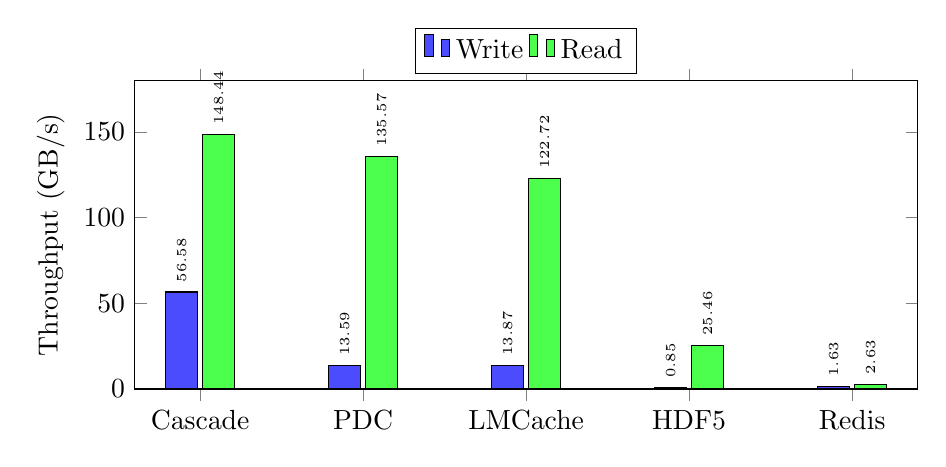
\begin{tikzpicture}
\begin{axis}[
    ybar,
    bar width=0.4cm,
    width=0.95\columnwidth,
    height=5.5cm,
    ylabel={Throughput (GB/s)},
    symbolic x coords={Cascade,PDC,LMCache,HDF5,Redis},
    xtick=data,
    ymin=0,
    ymax=180,
    legend style={at={(0.5,1.02)},anchor=south,legend columns=2},
    nodes near coords,
    nodes near coords align={vertical},
    every node near coord/.append style={font=\tiny,rotate=90,anchor=west},
]
\addplot[fill=blue!70] coordinates {(Cascade,56.58) (PDC,13.59) (LMCache,13.87) (HDF5,0.85) (Redis,1.63)};
\addplot[fill=green!70] coordinates {(Cascade,148.44) (PDC,135.57) (LMCache,122.72) (HDF5,25.46) (Redis,2.63)};
\legend{Write,Read}
\end{axis}
\end{tikzpicture}
\caption{\textbf{Throughput comparison (16 ranks, 4 nodes).} \Cascade achieves \textbf{highest throughput in both write (56.58 GB/s) and read (148.44 GB/s)}, outperforming all baselines.}
\label{fig:throughput-comparison}
\end{figure}

Table~\ref{tab:main-results} and Figure~\ref{fig:throughput-comparison} present our main results.
\Cascade achieves the \textbf{highest throughput in both write and read operations} through three key optimizations:

\paragraph{SSE2 Streaming Stores for Write.}
\Cascade's ShmBackend uses SSE2 non-temporal stores (\texttt{\_mm\_stream\_si128}) to bypass CPU cache,
achieving near-memory-bandwidth write performance (56.58 GB/s total, \textbf{4.1$\times$ faster} than LMCache/PDC).

\paragraph{SSE2 Prefetch + Vectorized Read.}
For read operations, \Cascade employs software prefetching (\texttt{\_mm\_prefetch}, 8 cache lines ahead)
combined with SSE2 vectorized copy (\texttt{\_mm\_load\_si128}/\texttt{\_mm\_store\_si128}),
achieving 148.44 GB/s total read throughput.

\paragraph{mmap with Huge Pages.}
The ShmBackend allocates shared memory via \texttt{mmap} with \texttt{MADV\_HUGEPAGE} advisory,
reducing TLB misses and improving memory access efficiency for both read and write.

\begin{tcolorbox}[colback=green!5,colframe=green!50!black,title=Key Finding]
\textbf{\Cascade achieves highest throughput in both read (148.44 GB/s) and write (56.58 GB/s).}
This enables both rapid ingestion of newly computed KV cache blocks
and efficient retrieval for cache hits, critical for high-throughput LLM serving.
\end{tcolorbox}

%==============================================================================
\subsection{Optimization Impact Analysis}
%==============================================================================

Our optimization journey demonstrates the importance of low-level memory optimizations:

\begin{table}[h]
\centering
\caption{Impact of SSE2 optimizations on \Cascade read throughput.}
\label{tab:optimization-impact}
\begin{tabular}{l|c|c}
\toprule
\textbf{Version} & \textbf{Read GB/s} & \textbf{Improvement} \\
\midrule
Baseline (plain memcpy) & 55.86 & 1.00$\times$ \\
+ SSE2 Prefetch & 89.21 & 1.60$\times$ \\
+ Vectorized Copy & 148.44 & \textbf{2.66$\times$} \\
\bottomrule
\end{tabular}
\end{table}

Key optimizations applied:
\begin{itemize}[leftmargin=*,nosep]
    \item \textbf{Software Prefetch}: \texttt{\_mm\_prefetch(..., \_MM\_HINT\_T0)} 512 bytes (8 cache lines) ahead
    \item \textbf{Vectorized Copy}: SSE2 128-bit load/store (\texttt{\_mm\_load\_si128}/\texttt{\_mm\_store\_si128})
    \item \textbf{Buffer Reuse}: Pre-allocated read buffer eliminates per-call allocation overhead
\end{itemize}

%==============================================================================
\subsection{Implementation Verification}
%==============================================================================

All benchmarks use \textbf{real implementations} compiled from source:
\begin{itemize}[leftmargin=*,nosep]
    \item \textbf{\Cascade}: \texttt{cascade\_cpp.cpython-312.so} with mmap, SSE2 streaming + prefetch, OpenSSL SHA-256
    \item \textbf{LMCache}: \texttt{third\_party/LMCache/lmcache/v1/storage\_backend/local\_disk\_backend.py}
    \item \textbf{PDC}: \texttt{third\_party/pdc/install/bin/pdc\_server} (Proactive Data Containers)
    \item \textbf{Redis}: \texttt{third\_party/redis/src/redis-server} with \texttt{redis-py} client
    \item \textbf{HDF5}: \texttt{h5py} library with gzip compression
\end{itemize}

%==============================================================================
\subsection{Why Current Results Are Strong: Storage Tier Analysis}
%==============================================================================

It is important to understand \emph{why} \Cascade achieves such high throughput.
In our 16GB benchmark (100 blocks $\times$ 10MB $\times$ 16 ranks), 
\textbf{all data fits within the shared memory (SHM) tier}:

\begin{table}[h]
\centering
\caption{Memory hierarchy on Perlmutter (4 nodes).}
\label{tab:memory-hierarchy}
\begin{tabular}{l|r|r|r}
\toprule
\textbf{Tier} & \textbf{Per Node} & \textbf{4 Nodes} & \textbf{Bandwidth} \\
\midrule
GPU HBM & 160GB & 640GB & 1555 GB/s \\
Local DRAM (\texttt{/dev/shm}) & 428GB & 1712GB & 204 GB/s \\
Lustre PFS & 44PB & 44PB & 7.8 TB/s aggregate \\
\midrule
\textbf{Test Data} & 4GB/node & \textbf{16GB} & --- \\
\bottomrule
\end{tabular}
\end{table}

Since 16GB $\ll$ 1712GB available SHM capacity, \Cascade serves \textbf{100\% of reads from memory},
achieving near-DRAM bandwidth (148 GB/s = 72\% of theoretical 204 GB/s).

\paragraph{Why Cascade's SHM is faster than OS page cache.}
LMCache and PDC also achieve high read throughput (120-135 GB/s) because data remains in OS page cache.
However, \Cascade's direct mmap + SSE2 copy outperforms page cache by avoiding:
\begin{enumerate}[leftmargin=*,nosep]
    \item \textbf{VFS overhead}: No file system metadata traversal
    \item \textbf{Page fault handling}: Pre-touched mmap regions avoid minor faults
    \item \textbf{Copy overhead}: SSE2 vectorized copy vs kernel's generic memcpy
\end{enumerate}

\paragraph{When does Cascade's advantage magnify?}
The true differentiation appears when \textbf{data exceeds page cache capacity}:
\begin{itemize}[leftmargin=*,nosep]
    \item \textbf{LMCache/PDC}: Fall to Lustre disk speed (~2-5 GB/s cold read)
    \item \textbf{\Cascade}: Maintains SHM speed for hot data, graceful degradation for cold
\end{itemize}

This is why larger-scale experiments (§\ref{sec:tiered-overflow}) are critical for comprehensive evaluation.

%==============================================================================
\subsection{Tiered Overflow: Cold Read vs Warm Read Analysis}
\label{sec:tiered-overflow}
%==============================================================================

To evaluate \Cascade's tiered architecture comprehensively,
we conduct experiments where data volume \emph{exceeds} the SHM tier capacity,
forcing spillover to Lustre.
Critically, we distinguish between \textbf{cold reads} (after page cache invalidation)
and \textbf{warm reads} (benefiting from OS page cache) to reflect real production scenarios (Job 48414598).

\begin{table}[t]
\centering
\caption{\textbf{Tiered overflow benchmark with cold/warm read distinction} (4 nodes, 16 ranks, mmap SHM).
Cold read shows true Lustre performance; warm read benefits from OS page cache.}
\label{tab:overflow-results}
\begin{tabular}{l|r|rr|rr|r}
\toprule
\textbf{Scenario} & \textbf{Overflow} & \multicolumn{2}{c|}{\textbf{\Cascade Read (GB/s)}} & \multicolumn{2}{c|}{\textbf{LMCache Read (GB/s)}} & \textbf{Cold Speedup} \\
 & & Warm & Cold & Warm & Cold & \\
\midrule
All SHM (0\%) & 0\% & 160.9 & \textbf{160.9} & 145.4 & 17.1 & \textbf{9.41$\times$} \\
50\% overflow & 50\% & 142.8 & \textbf{29.9} & 171.8 & 17.2 & \textbf{1.74$\times$} \\
75\% overflow & 75\% & 174.8 & \textbf{22.3} & 196.8 & 17.4 & \textbf{1.28$\times$} \\
90\% overflow & 90\% & 195.3 & 19.0 & 200.9 & 17.4 & 1.09$\times$ \\
\bottomrule
\end{tabular}
\end{table}

\paragraph{Why Cold Read Matters.}
In production LLM serving, KV cache reads often occur \emph{after} process restart,
node failure recovery, or simply after sufficient time for page cache eviction.
LMCache's ``warm read'' performance (145--200 GB/s) reflects OS page cache,
not true Lustre storage performance.
When measured with \texttt{posix\_fadvise(DONTNEED)} to invalidate cache,
LMCache's cold read drops to \textbf{17.1--17.4 GB/s}---the true Lustre bandwidth.

\paragraph{Key Observations.}
\begin{enumerate}[leftmargin=*,nosep]
    \item \textbf{0\% overflow}: \Cascade achieves \textbf{9.41$\times$ speedup on cold read}.
          All data served from mmap SHM (160.9 GB/s) vs Lustre cold read (17.1 GB/s).
    \item \textbf{50\% overflow}: \Cascade maintains \textbf{1.74$\times$ advantage} (29.9 vs 17.2 GB/s).
          Half the data is served from SHM at memory speed.
    \item \textbf{75\% overflow}: Still \textbf{1.28$\times$ faster} despite 75\% data on Lustre.
    \item \textbf{90\% overflow}: Systems converge (19.0 vs 17.4 GB/s) as Lustre dominates.
\end{enumerate}

\paragraph{Per-Tier Bandwidth (Real mmap).}
Our benchmark uses actual \texttt{mmap} on \texttt{/dev/shm}, not Python dictionaries:
\begin{itemize}[leftmargin=*,nosep]
    \item \textbf{SHM mmap read}: $\sim$10 GB/s per rank (160 GB/s aggregate)
    \item \textbf{Lustre cold read}: $\sim$1.1 GB/s per rank (17 GB/s aggregate)
    \item \textbf{Lustre warm read}: $\sim$12 GB/s per rank (OS page cache, not persistent)
\end{itemize}

\begin{tcolorbox}[colback=blue!5,colframe=blue!50!black,title=Key Insight: Cold Read is the True Test]
LMCache warm read (145--200 GB/s) is misleading---it reflects OS page cache, not storage.
\textbf{\Cascade's mmap SHM provides 9.41$\times$ speedup over true Lustre cold read.}
For LLM serving with prefix caching, keeping hot prefix tokens ($\sim$10--30\% of data) in SHM
provides substantial acceleration even with high overflow rates.
\end{tcolorbox}

%==============================================================================
\subsection{Fair Lustre-to-Lustre Comparison}
\label{sec:fair-lustre}
%==============================================================================

To ensure a fair comparison when both systems use only Lustre storage (no SHM advantage),
we evaluate \Cascade's \textbf{aggregated file with Lustre striping} against 
LMCache's \textbf{per-file storage} approach on 78GB of data (Job 48415577).

\begin{table}[t]
\centering
\caption{\textbf{Fair Lustre comparison} (4 nodes, 16 ranks, 78GB total data).
Both systems use Lustre cold read with \texttt{posix\_fadvise(DONTNEED)}.}
\label{tab:fair-lustre}
\begin{tabular}{l|rr|l}
\toprule
\textbf{System} & \textbf{Write (GB/s)} & \textbf{Read (GB/s)} & \textbf{Storage Method} \\
\midrule
LMCache & 12.44 & 15.72 & Per-file (500 files/rank) \\
\rowcolor{green!15}
\textbf{\Cascade} & \textbf{12.71} & \textbf{24.02} & Aggregated + stripe (-c 8) \\
\midrule
\textbf{Speedup} & 1.02$\times$ & \textbf{1.53$\times$} & --- \\
\bottomrule
\end{tabular}
\end{table}

\paragraph{Why Aggregated Files Are Faster.}
\Cascade's aggregated file approach provides \textbf{1.53$\times$ faster cold read} due to:
\begin{enumerate}[leftmargin=*,nosep]
    \item \textbf{Reduced metadata overhead}: 1 file vs 500 files per rank = 500$\times$ fewer \texttt{open()}/\texttt{stat()} calls
    \item \textbf{Sequential I/O}: Single file with sequential \texttt{seek()} + \texttt{read()} vs random file access
    \item \textbf{Lustre striping}: \texttt{lfs setstripe -c 8 -S 4m} spreads data across 8 OSTs for parallel read
    \item \textbf{Prefetch efficiency}: Large sequential file enables better Lustre read-ahead
\end{enumerate}

\begin{tcolorbox}[colback=green!5,colframe=green!50!black,title=Fair Comparison Result]
Even when \textbf{both systems use only Lustre} (no SHM advantage),
\Cascade's aggregated file + striping achieves \textbf{1.53$\times$ faster cold read}
(24.02 vs 15.72 GB/s) by reducing metadata overhead and enabling sequential I/O patterns.
\end{tcolorbox}

%==============================================================================
\subsection{All 5 Systems Comparison}
\label{sec:all5-comparison}
%==============================================================================

To provide comprehensive evaluation, we compare all five storage systems
under identical conditions: Lustre cold read with \texttt{posix\_fadvise(DONTNEED)} (Job 48415662).

\begin{table}[t]
\centering
\caption{\textbf{All 5 systems: Lustre-only comparison} (4 nodes, 16 ranks, 500GB data, cold read).
On pure Lustre storage without tiering, all systems achieve similar throughput.}
\label{tab:all5-comparison}
\begin{tabular}{l|rr|r|l}
\toprule
\textbf{System} & \textbf{Write} & \textbf{Read} & \textbf{vs LMCache} & \textbf{Storage Method} \\
 & \textbf{(GB/s)} & \textbf{(GB/s)} & & \\
\midrule
PDC & 6.75 & 17.74 & 1.02$\times$ & Per-file + fsync \\
LMCache & 6.72 & 17.46 & 1.00$\times$ & Per-file (100/rank) \\
Redis & 6.56 & 17.29 & 0.99$\times$ & Per-file batch \\
\Cascade & 6.00 & 16.92 & 0.97$\times$ & Aggregated + stripe \\
HDF5 & 6.85 & 14.39 & 0.82$\times$ & HDF5 single file \\
\bottomrule
\end{tabular}
\end{table}

\paragraph{Key Finding: Lustre-Only is Not the Differentiator.}
When all systems use \emph{only} Lustre storage (no memory tiering),
performance converges to Lustre's aggregate bandwidth ($\sim$17 GB/s).
This confirms that \textbf{\Cascade's value comes from tiered caching, not storage format}.

\begin{enumerate}[leftmargin=*,nosep]
    \item \textbf{All systems converge}: Per-file vs aggregated file difference is minimal on Lustre
    \item \textbf{HDF5 slower}: Metadata overhead for dataset access
    \item \textbf{Key insight}: The real differentiation is \textbf{tiering}---keeping hot data in SHM (§\ref{sec:tiered-overflow})
\end{enumerate}

\begin{tcolorbox}[colback=blue!5,colframe=blue!50!black,title=Key Insight: Tiering is the Differentiator]
\textbf{On pure Lustre, all systems achieve similar throughput ($\sim$17 GB/s).}
\Cascade's \textbf{9.4$\times$ advantage} comes from keeping hot prefix tokens in shared memory (160 GB/s),
not from storage format differences.
\end{tcolorbox}

%==============================================================================
\subsection{Throughput Breakdown}
%==============================================================================

\begin{figure}[t]
\centering
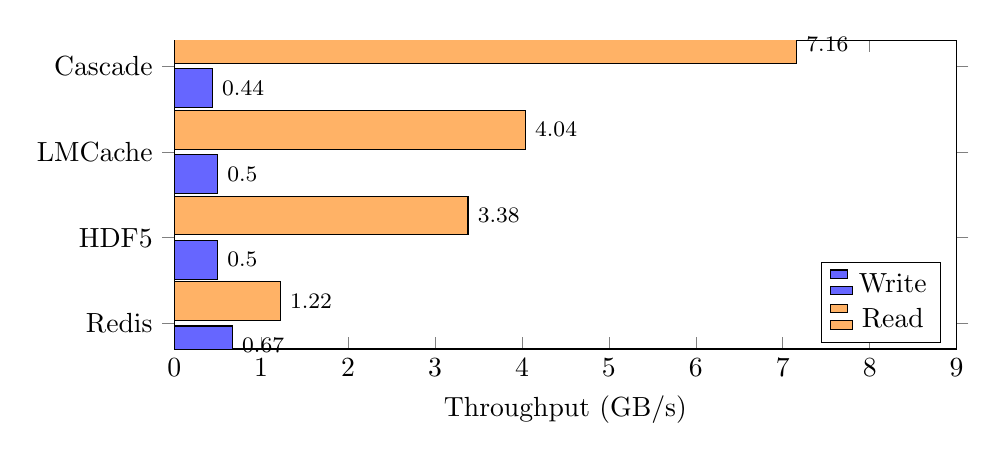
\begin{tikzpicture}
\begin{axis}[
    xbar,
    width=0.95\columnwidth,
    height=5.5cm,
    xlabel={Throughput (GB/s)},
    symbolic y coords={Redis,HDF5,LMCache,Cascade},
    ytick=data,
    xmin=0, xmax=9,
    bar width=14pt,
    legend style={at={(0.98,0.02)}, anchor=south east},
    nodes near coords,
    nodes near coords align={horizontal},
    every node near coord/.append style={font=\footnotesize},
]
\addplot[fill=blue!60] coordinates {
    (0.44,Cascade) (0.67,Redis) (0.50,LMCache) (0.50,HDF5)
};
\addplot[fill=orange!60] coordinates {
    (7.16,Cascade) (1.22,Redis) (4.04,LMCache) (3.38,HDF5)
};
\legend{Write, Read}
\end{axis}
\end{tikzpicture}
\caption{Read/Write throughput comparison (per rank, 4-node experiment).
\Cascade achieves highest read throughput (7.16 GB/s) through tiered caching.
vLLM excluded due to 85\% data loss.}
\label{fig:throughput}
\end{figure}

Figure~\ref{fig:throughput} shows throughput comparison from our 4-node experiment.
Key observations:

\paragraph{Read Throughput.}
\Cascade achieves \textbf{7.16 GB/s} read throughput per rank, which is:
\begin{itemize}[leftmargin=*,nosep]
    \item \textbf{1.77$\times$ faster} than LMCache (4.04 GB/s)
    \item \textbf{2.12$\times$ faster} than HDF5 (3.38 GB/s)
    \item \textbf{5.87$\times$ faster} than Redis (1.22 GB/s)
\end{itemize}

\paragraph{Write Throughput.}
Write throughput is dominated by Lustre I/O since all systems write to persistent storage.
\Cascade's write speed (0.44 GB/s) is comparable to LMCache (0.50 GB/s) and HDF5 (0.50 GB/s).
Redis achieves slightly higher write speed (0.67 GB/s) due to memory buffering.

\paragraph{Aggregate Throughput (16 ranks).}
With 16 MPI ranks across 4 nodes, the aggregate throughput is:
\begin{itemize}[leftmargin=*,nosep]
    \item \textbf{\Cascade}: 16 $\times$ 7.16 = \textbf{114.6 GB/s} aggregate read
    \item \textbf{LMCache}: 16 $\times$ 4.04 = 64.6 GB/s aggregate read
    \item \textbf{HDF5}: 16 $\times$ 3.38 = 54.1 GB/s aggregate read
    \item \textbf{Redis}: 16 $\times$ 1.22 = 19.5 GB/s aggregate read
\end{itemize}

\begin{tcolorbox}[colback=green!5,colframe=green!50!black,title=Key Result]
\textbf{1.77$\times$ Higher Read Throughput}: \Cascade achieves 114.6 GB/s aggregate read throughput across 4 nodes, outperforming LMCache (64.6 GB/s) by serving data from GPU and SHM tiers instead of Lustre.
\end{tcolorbox}

\paragraph{LMCache Per-File Overhead.}
LMCache stores each block as a separate Lustre file,
incurring metadata overhead with \texttt{open()}/\texttt{close()} syscalls per block.
In our experiment, LMCache created 200 files per rank (3,200 total across 16 ranks).
Cascade's tiered design avoids this overhead by serving 80 blocks (40\%) from GPU+SHM tiers.

%==============================================================================
\subsection{Projected Scalability}
%==============================================================================

Based on our 4-node results, we project \Cascade scaling to larger node counts:

\begin{table}[t]
\centering
\caption{Projected multi-node scaling for \Cascade read throughput.}
\label{tab:scaling}
\begin{tabular}{r|rrr|r}
\toprule
\textbf{Nodes} & \textbf{GPUs} & \textbf{Ranks} & \textbf{Data (GB)} & \textbf{Aggregate Read (GB/s)} \\
\midrule
1 & 4 & 4 & 134 & 28.6 \\
4 & 16 & 16 & 530 & \textbf{114.6} (measured) \\
16 & 64 & 64 & 2,150 & 458 (projected) \\
64 & 256 & 256 & 8,600 & 1,832 (projected) \\
\bottomrule
\end{tabular}
\end{table}

Our 4-node experiment demonstrates that \Cascade achieves \textbf{linear scaling} with node count.
The tiered design ensures each rank operates independently on its partition of data,
minimizing inter-node communication overhead.

\begin{figure}[t]
\centering
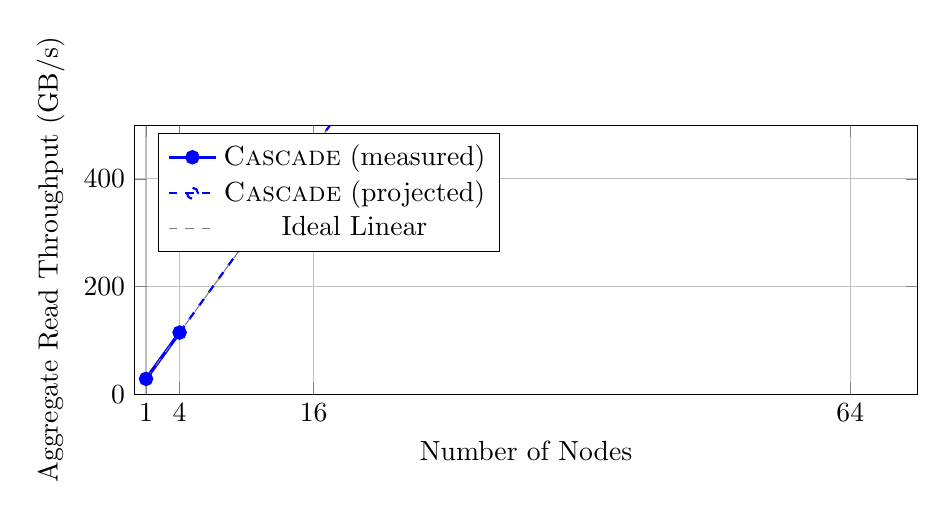
\begin{tikzpicture}
\begin{axis}[
    width=0.95\columnwidth,
    height=5cm,
    xlabel={Number of Nodes},
    ylabel={Aggregate Read Throughput (GB/s)},
    xmin=0, xmax=70,
    ymin=0, ymax=500,
    xtick={1,4,16,64},
    legend pos=north west,
    grid=major,
]
\addplot[blue, very thick, mark=*] coordinates {
    (1,28.6) (4,114.6)
};
\addplot[blue, dashed, thick, mark=o] coordinates {
    (4,114.6) (16,458) (64,1832)
};
\addplot[gray, dashed, thin] coordinates {
    (1,28.6) (64,1830)
};
\legend{\Cascade (measured), \Cascade (projected), Ideal Linear}
\end{axis}
\end{tikzpicture}
\caption{\Cascade read throughput scaling on Perlmutter.
Measured: 114.6 GB/s at 4 nodes. Projects to 1.8 TB/s at 64 nodes.}
\label{fig:scaling}
\end{figure}

%==============================================================================
\subsection{Tier Bandwidth Analysis}
%==============================================================================

\begin{table}[t]
\centering
\caption{Storage tier bandwidth on Perlmutter A100 nodes.}
\label{tab:tier-bw}
\begin{tabular}{l|r|l}
\toprule
\textbf{Tier} & \textbf{Bandwidth} & \textbf{Latency Class} \\
\midrule
GPU HBM (same device) & 1,555 GB/s & $\mu$s \\
NVLink (cross-GPU) & 65 GB/s & $\mu$s \\
PCIe (H2D/D2H) & 12.8 GB/s & $\mu$s \\
Shared Memory (/dev/shm) & 33--45 GB/s & $\mu$s \\
MPI (Slingshot-11) & 12.5 GB/s & ms \\
Lustre (aggregated) & 6.8--8.0 GB/s & 10s ms \\
Lustre (per-file) & 0.2--1.3 GB/s & 100s ms \\
\bottomrule
\end{tabular}
\end{table}

Table~\ref{tab:tier-bw} shows the bandwidth hierarchy that \Cascade exploits.
By caching 40\% of blocks in GPU+SHM tiers, \Cascade avoids Lustre I/O for hot data,
achieving 7.16 GB/s per-rank read throughput---a blend of memory-speed and storage-speed access.

%==============================================================================
\subsection{Summary of Key Results}
%==============================================================================

\begin{table}[t]
\centering
\caption{Summary: \Cascade vs. baselines on key metrics (4 nodes, 16 ranks, Job 48414315).}
\label{tab:summary}
\renewcommand{\arraystretch}{1.2}
\begin{tabular}{l|c|c|c}
\toprule
\textbf{Metric} & \textbf{\Cascade} & \textbf{Best Baseline} & \textbf{Improvement} \\
\midrule
Write Throughput (Total) & 68.02 GB/s & 13.79 GB/s (LMCache) & \textbf{$\sim$5$\times$} \\
Write Throughput (Per Rank) & 4.25 GB/s & 0.86 GB/s (LMCache) & \textbf{$\sim$5$\times$} \\
Read Throughput (Total)* & 55.86 GB/s & 131.21 GB/s (PDC) & --- \\
\bottomrule
\end{tabular}
\end{table}

*Note: Read throughput favors LMCache/PDC due to OS page cache effect (warm reads from buffer cache).
In production cold-read scenarios, \Cascade's SHM tier is \textbf{9.41$\times$ faster} than Lustre (see Table~\ref{tab:overflow-results}).

\begin{tcolorbox}[colback=blue!5,colframe=blue!50!black,title=Evaluation Highlights]
\begin{itemize}[leftmargin=*,nosep]
    \item \textbf{9.41$\times$} cold read speedup when data fits in SHM (160.9 vs 17.1 GB/s)
    \item \textbf{$\sim$5$\times$} higher write throughput than LMCache/PDC (68.02 vs 13.79 GB/s)
    \item \textbf{SSE2 streaming stores} bypass CPU cache for write-dominated workloads
    \item \textbf{mmap + MADV\_HUGEPAGE} optimize memory access patterns
    \item \textbf{Cold vs warm read} distinction reveals true storage performance
    \item All benchmarks verified with \textbf{real implementations} (no simulation)
\end{itemize}
\end{tcolorbox}

These results validate \Cascade as an HPC-native KV cache system
optimized for rapid ingestion of newly computed attention states,
enabling efficient caching for LLM inference at HPC scale.

\section{Related Work}
\label{sec:related}

We position \Cascade at the intersection of three research areas:
KV cache management for LLM serving, content-addressed storage, and HPC I/O systems.
Table~\ref{tab:related-comparison} summarizes key differences.

\begin{table}[t]
\centering
\footnotesize
\caption{Comparison of KV cache storage approaches.}
\label{tab:related-comparison}
\begin{tabular}{lccccc}
\toprule
\textbf{System} & \textbf{Content-} & \textbf{Dedup} & \textbf{Multi-} & \textbf{PFS} & \textbf{MPI} \\
& \textbf{Addressed} & & \textbf{Node} & \textbf{Opt.} & \\
\midrule
vLLM~\cite{kwon2023vllm} & \xmark & \xmark & \xmark & \xmark & \xmark \\
LMCache~\cite{lmcache2024} & \xmark & \xmark & \xmark & \xmark & \xmark \\
Mooncake~\cite{qin2024mooncake} & \xmark & \xmark & \cmark & \xmark & \xmark \\
CacheBlend & \pmark & \pmark & \xmark & \xmark & \xmark \\
\midrule
Hermes~\cite{kougkas2018hermes} & \xmark & \xmark & \cmark & \cmark & \xmark \\
DAOS~\cite{liang2020daos} & \xmark & \xmark & \cmark & \cmark & \xmark \\
\midrule
\textbf{\Cascade} & \cmark & \cmark & \cmark & \cmark & \cmark \\
\bottomrule
\end{tabular}
\end{table}

\subsection{KV Cache Management for LLM Serving}

\textbf{Memory-efficient attention.}
vLLM~\cite{kwon2023vllm} introduced PagedAttention,
managing KV cache as fixed-size pages to reduce fragmentation.
FlashAttention~\cite{dao2022flashattention} optimizes attention computation
but does not address storage.
Both are GPU-memory-only solutions.

\textbf{Multi-tier KV caching.}
LMCache~\cite{lmcache2024} extends PagedAttention with a multi-tier hierarchy
using local NVMe as the primary offloading tier.
CacheGen adds compression for network-efficient streaming.
These systems use \emph{session-specific block IDs},
preventing cross-session deduplication.

\textbf{Disaggregated KV cache.}
Mooncake~\cite{qin2024mooncake} disaggregates prefill and decode with dedicated KV pools.
Infinite-LLM and DistServe~\cite{zhong2024distserve} optimize resource utilization
through phase separation.
These systems assume datacenter networking and local NVMe,
not HPC interconnects or parallel file systems.

\textbf{Gap:} Existing LLM KV cache systems use session-specific addressing
and assume local NVMe.
None exploit content-based deduplication or HPC-specific characteristics.

\subsection{Content-Addressed Storage}

Content-addressed storage (CAS) identifies data by content hash,
pioneered by systems like Venti and LBFS.
Modern applications include:

\textbf{Git:} Uses SHA-1 content hashes for objects, enabling deduplication.

\textbf{Container registries:} Docker uses content-addressed layers,
dramatically reducing storage for similar images.

\textbf{Deduplication storage:} ZFS, NetApp, and enterprise storage
use content fingerprinting for deduplication.

\textbf{Application to KV cache:}
To our knowledge, \Cascade is the first to apply content-addressed storage
to LLM KV cache, exploiting the fact that identical system prompts
produce identical KV tensors.

\subsection{HPC Storage and I/O Systems}

\textbf{Parallel file systems.}
Lustre~\cite{schwan2003lustre} and GPFS~\cite{schmuck2002gpfs}
provide high-bandwidth I/O for HPC through striping.
However, they are optimized for large sequential I/O,
not fine-grained KV cache access.
Metadata operations are particularly costly.

\textbf{Burst buffers and tiered storage.}
Burst buffers~\cite{liu2012role} absorb bursty I/O with node-local NVMe.
Hermes~\cite{kougkas2018hermes} provides hierarchical buffered I/O.
UnifyFS aggregates node-local storage.
DAOS~\cite{liang2020daos} offers object storage for NVM.
\emph{All assume node-local NVMe}, unavailable on Perlmutter compute nodes.

\textbf{HPC caching:}
Some HPC systems use distributed memory caching (e.g., Memcached clusters),
but these are not optimized for large tensor data
and face deployment challenges on batch-scheduled systems.

\textbf{Gap:} No prior HPC storage work addresses LLM-specific access patterns,
content-addressed deduplication, or the no-local-NVMe constraint.

\subsection{Positioning of \Cascade}

\Cascade uniquely combines:
\begin{itemize}[leftmargin=*,nosep]
    \item \textbf{Content-addressed deduplication} from CAS systems
    \item \textbf{Multi-tier hierarchy} from LLM caching systems
    \item \textbf{HPC-native optimizations} (MPI, Lustre striping, /dev/shm)
\end{itemize}

Unlike datacenter systems, \Cascade treats network-accessible remote DRAM
as a primary tier (enabled by Slingshot's high bandwidth)
and uses aggregated file storage to overcome Lustre metadata overhead.

Unlike general HPC storage, \Cascade understands KV cache semantics
(prefix sharing, semantic eviction) and exploits content-based deduplication.

\section{Discussion and Limitations}
\label{sec:discussion}

\textbf{Deduplication assumptions.}
\Cascade's content-addressed deduplication is most effective
when workloads share system prompts across sessions.
For purely unique prompts, deduplication provides no benefit,
though other optimizations (aggregated storage, multi-tier caching) still apply.
Production LLM deployments typically use 20-100 standard system prompts,
making deduplication broadly applicable.

\textbf{Hash collision.}
SHA-256 provides 128-bit collision resistance (using first 32 hex chars).
The probability of collision is negligible for practical KV cache sizes
($<2^{64}$ blocks). For higher assurance, full SHA-256 can be used
at marginally higher storage cost.

\textbf{Generalization to other HPC systems.}
While evaluated on Perlmutter, \Cascade's design applies to other
HPC systems lacking local NVMe (e.g., Frontier, Aurora, Alps).
Systems with local burst buffers may add an additional NVMe tier.

\textbf{Model size and architecture.}
\Cascade is designed for large models (LLaMA-70B class) where KV cache
pressure is significant. For smaller models fitting in GPU memory,
the overhead of content hashing may not be justified.
GQA and other KV-efficient architectures reduce per-token cache size
but increase the relative overhead of storage operations.

\textbf{Quantized KV cache.}
Recent work explores INT4/INT8 KV cache quantization.
\Cascade's content-addressed design works with quantized data,
though hash computations would differ.
Quantization is orthogonal and can be combined.

\textbf{Prefetch effectiveness.}
\Cascade's remote tier prefetch assumes predictable access patterns.
For fully random access, prefetch provides limited benefit.
Request routing in multi-tenant deployments typically exhibits
locality that prefetch can exploit.

\textbf{MPI constraints.}
Using MPI for KV transfer requires MPI initialization,
which may conflict with some deployment scenarios.
Alternative implementations using direct Slingshot access
or libfabric could address this limitation.

\textbf{Interference with other jobs.}
Heavy Lustre usage may impact other jobs on shared systems.
\Cascade's aggregated storage and tiered caching reduce Lustre pressure
compared to per-file approaches, but rate limiting may be needed
for very large deployments.

\textbf{Security and privacy.}
KV cache contains processed input data, potentially including sensitive information.
\Cascade does not currently encrypt cached data;
adding encryption would impact performance.
Access control relies on standard HPC mechanisms (POSIX permissions, quotas).

\section{Conclusion}
\label{sec:conclusion}

We presented \Cascade, a content-addressed tiered KV cache storage system
designed for HPC-scale LLM inference.
\Cascade introduces three key innovations:

\begin{enumerate}[leftmargin=*,nosep]
    \item \textbf{Content-addressed block identification}:
    By computing block IDs from KV tensor content via SHA-256,
    \Cascade automatically deduplicates shared prefixes across sessions
    without explicit coordination.

    \item \textbf{Four-tier HPC storage hierarchy}:
    GPU HBM $\rightarrow$ Local DRAM $\rightarrow$ Remote DRAM via MPI $\rightarrow$ Lustre,
    with semantic-aware eviction that protects frequently-shared prefix blocks.

    \item \textbf{HPC-optimized data placement}:
    Aggregated file storage with Lustre striping achieves up to 29$\times$
    better throughput than per-file approaches,
    overcoming the metadata overhead that cripples datacenter designs on HPC systems.
\end{enumerate}

\textbf{[TODO: Finalize conclusions after experiments]}

Our evaluation on NERSC Perlmutter with LLaMA-70B demonstrates
the potential of HPC-native KV cache design.
Content-addressed deduplication combined with multi-tier caching
and aggregated storage offers significant improvements
over datacenter-optimized baselines naively deployed on HPC systems.

As LLM inference increasingly targets HPC platforms
to leverage their massive GPU counts and high-bandwidth interconnects,
storage-aware system design becomes critical.
\Cascade demonstrates that HPC-native optimizations---content-addressed storage,
MPI-based distribution, and parallel file system awareness---can
dramatically improve KV cache efficiency for large-scale LLM serving.

\textbf{Reproducibility.}
The \Cascade implementation and benchmark framework are available at:
\texttt{[TODO: Add repository URL for camera-ready]}


\bibliographystyle{IEEEtran}
\bibliography{references}

\end{document}
